\pdfbookmark{\tth Application}{ttH_dilep application}
\chapter{\tth Application}
\label{Application}

\begin{quote}
\textit{The \tth application for event reconstruction is presented in this chapter. Its dependencies are presented. The flow of the application is presented in section \ref{Application:Flow}, accompanied by a schematic representation. Its main functions are presented and the schematic flow is compared against a callgraph of the application to help understanding what happens in each of the most important functions. The critical region is identified in section \ref{CriticalRegion} and characterized in subsection \ref{ComputationalCharactrization}. Some initial optimizations to the code are presented in subsection \ref{InitialOptimizations}.}
\end{quote}

The LIP research group developed the \tth application to solve the problem presented in section \ref{Motivation}, which runs in the Tier-3 CERN computational resources. Its name derived from the problem it was design to solve: the \textit{tt} is relative to the reconstruction of the \ttbar system; the \textit{H} is derived from the Higgs boson reconstruction; the \textit{dilep} is the name of the function responsable for the kinematical reconstruction, as it needs two leptons (di-lep) as input.

The application has two main dependencies in external libraries. The most important is on ROOT \cite{CERN:ROOT}, a object oriented framework, developed at CERN, which provides a set of funcionalities oriented for handling, analyzing and displaying results for large amounts of data collected at the LHC. It provides an API for reading and storing data in the standard formats accepted by all the tiers centers, classes for representing physic elements, mathematical routines, pseudorandom number generators, histograming, curve fitting minimization and data visualization methods. It is originally designed and developed mostly by physicists self taught on programming. This results in a framework that has room for improvement, such as code restructuration in some modules related to the data analysis. Other possible optimizations could pass through replacing some mathematical functionalities by dependencies on faster libraries, such as BLAS \cite{BLAS} or MKL \cite{MKL}. ROOT has an extension for data distribution on distributed memory systems, the Parallel ROOT Facility (PROOF) \cite{CERN:PROOF}.

The second dependency is on the LipMiniAnalysis library. It is a modified version of LipCbrAnalysis, a library developed LIP for in-house use, which provides a skeleton (not an API) for creating an analysis application. It provides a set of functions that are common ground for most applications developed by LIP. This library is currently not suited for parallelization in shared or distributed memory, as later explained in chapter \ref{ParallelizationApproaches}.

During the following sections will be presented the flow of the application and an early profiling, identifying and characterizing the bottlenecks.

\pdfbookmark{Application Flow}{application flow}
\section{Application Flow}
\label{Application:Flow}

This section describes the workflow of the \tth analysis. The application flow is schematized in figure \ref{fig:SchematicFlow1}. It has two main elements, which are repeated for every event in the input data file: 

\begin{description}
	\item[\textit{Load Event Data:}] information relative to the event, all the Bottom Quark jets and leptons characteristics, as well as other control data, are loaded to a global state. Most of this state belongs to the LipMiniAnalysis and it is overwritten every time a new event is loaded. The function responsible for loading and processing an event is named \ttLoop.
	\item[\textit{Process Event:}] most of the event processing is performed in the \ttDoCuts function. In this function an event is tested in a set of filters (referred as cuts), with the possibility of being rejected in any of them and other event is loaded. This cuts test many characteristics of the events, such as the number of isolated leptons with opposite signs, the number of jets and the value of the particles masses. Only the events that reach cut number 20 are fit for the \ttbar system and Higgs boson reconstructions, which are computed in this filter by the complex \ttDilepKinFit. From a computational point of view, all the other cuts are simple.
	\item[\ttDilepKinFit:] this is the function responsible for the event reconstruction. It has an outer loop that iterates through all the possible combinations of 2 Bottom Quark jets and 2 leptons. The combination to process is determined and there is an inner loop that iterates through the number of variations per combination defined at compile time. The next step is to apply the variation to the particles characteristics and then the it attempts to reconstruct \ttbar system (kinematical reconstruction). If a reconstruction is possible, then the Higgs Boson is reconstructed and the probability of the reconstruction computed. If not, the reconstruction of that variation is discarded, as it is needed to know which jets were used in this reconstruction to avoid using them in the Higgs Boson reconstruction. The probability depends on the accuraccy of the kinematical and Higgs Boson reconstructions. Most of the data manipulated by this cut is stored in the global state of LipMiniAnalysis.
\end{description}

\begin{figure}[!htp]
	\begin{center}
		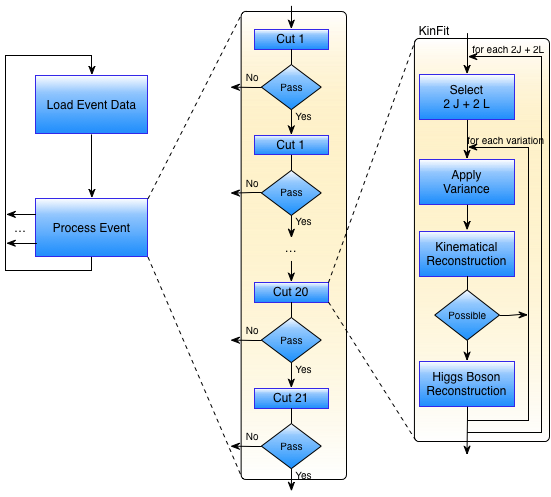
\includegraphics[scale=0.5]{../../common/img/graf_abstract_flow_with_kinfit.png}
		\caption{Schematic representation for the \tth application flow.}
		\label{fig:SchematicFlow1}
	\end{center}
\end{figure}

This schematic representation of the application flow was designed based on the source code analysis and the callgraphs obtained by using the callgrind tool from Valgrind \cite{Valgrind}. Besides giving an inside of the application structure, this tool provides simple profiling information, measuring how much percentage of time is spent in each function, which is very useful for a rough assement of the possible bottlenecks. The callgraph for the application is presented in figure \ref{fig:Callgraph1} and, since the objective is to run as many variations per combination, within a reasonable time frame, as explained in section \ref{Motivation}, a callgraph for 256 variations is presented in figure \ref{fig:Callgraph256}. Note that only the relevant functions are included in the callgraphs below, as the originals are much larger.

\begin{figure}[!htp]
	\begin{center}
		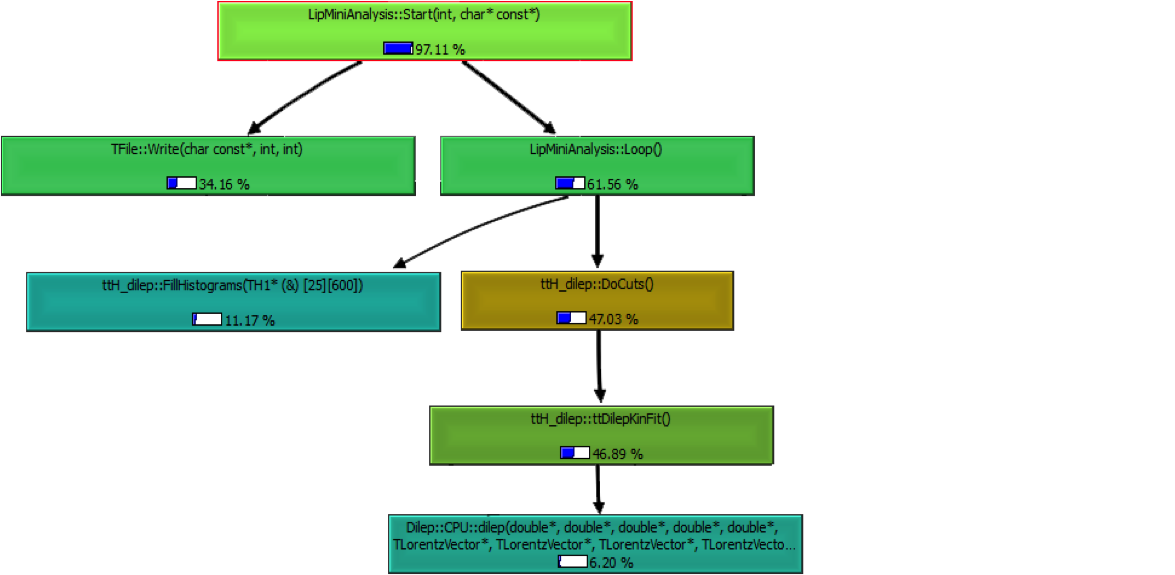
\includegraphics[scale=0.5]{../../common/img/callgraph_start_1.png}
		\caption{Callgraph for the \tth application on the compute-711 node\footnote{See appendix \ref{App:TestEnv} for characterization of all the systems used.}.}
		\label{fig:Callgraph1}
	\end{center}
\end{figure}

\begin{figure}[!htp]
	\begin{center}
		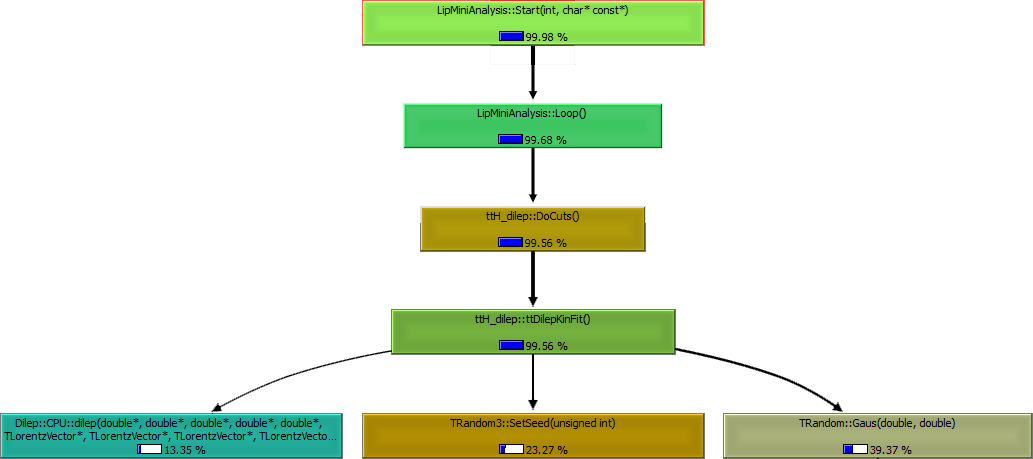
\includegraphics[scale=0.5]{../../common/img/callgraph_start_256.png}
		\caption{Callgraph for the \tth application on the compute-711 node for 256 variations per combination.}
		\label{fig:Callgraph256}
	\end{center}
\end{figure}

When performing only one variation per combination a third of the execution time is spent in writing outputs to files, using the ROOT library (note that all classes with a capital \textit{T} as prefix belong to ROOT) and the rest is spent processing the events. The cut number 20, \ttDilepKinFit, occupies most of the event processing time, where only 6.2\% of the time is on the kinematical reconstruction (\dilep). It is clear that the most complex cut is the portion of the application that must be optimized as it uses most of the execution time. This becomes even more evident when considering 256 variations per event, where \ttDilepKinFit uses 99.6\% of the application execution time. Now, it is possible to see that the pseudo-random number generator (\texttt{TRandom} and \texttt{TRandom3} classes) is taking a substantial part of the cut execution. Table \ref{tab:TempoKinFit} presents the percentage of the application execution time spent on \ttDilepKinFit, for various variations per combination. In section \ref{CriticalRegion} a computational analysis of the critical region is presented, as well as some early optimizations to the application.

\begin{table}[!htp]
	\begin{center}
		\begin{tabular}{|c|c|c|c|c|c|c|c|c|c|c|}
			\hline
			\textbf{# of variations/combination} & 1 & 2 & 4 & 8 & 16 & 32 & 64 & 128 & 256 & 512 \\ \hline
			\textbf{\% of time} & 46.9 & 62 & 76.9 & 87 & 92.9 & 96.3 & 98 & 98.9 & 99.6 & 99.7 \\ \hline
		\end{tabular}
		\caption{Percentage of the total execution time spent on the \ttDilepKinFit function for various numbers of variations per combination.}
		\label{tab:TempoKinFit}
	\end{center}
\end{table}

\section{Critical region computational characterization \& optimization}
\label{CriticalRegion}

This section will focus on the computational characterization of the \ttDilepKinFit function. It will be analyzed in terms of instruction mix, arithmetic and computational intensity and miss rate, with the purpose of understanding how this region of the code behaves, for various variations per combination, and classify it as a memory or compute bound algorithm. The test system used in this section is the compute-711\footnote{See appendix \ref{App:TestEnv} for characterization of all the systems used.}. Some initial optimizations, as well as other changes, made to the original application will be addressed in section \ref{InitialOptimizations}.

\subsection{Computational characterization}
\label{ComputationalCharactrization}

The \ttDilepKinFit, often referred as KinFit, is the most time consuming task in \tth application. Figure \ref{fig:KinFitGraph} presents the evolution of the absolute and relative execution time of the KinFit function, the I/O of the application, which was also identified by the callgraph \ref{fig:Callgraph1} as a time consuming task for a low number of variations, and the rest of the computations.

\begin{figure}
	\centering
	\begin{minipage}{.5\textwidth}
		\centering
		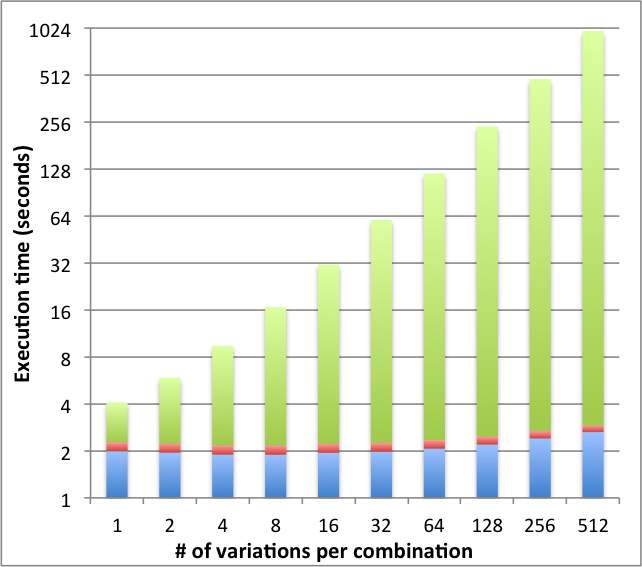
\includegraphics[scale=0.6]{../../common/graphs/exec_time_kinfit_rest.png}
	%	\captionof{figure}{A figure}
	%	\label{fig:KinFitGraph1}
	\end{minipage}%
	\begin{minipage}{.5\textwidth}
		\centering
		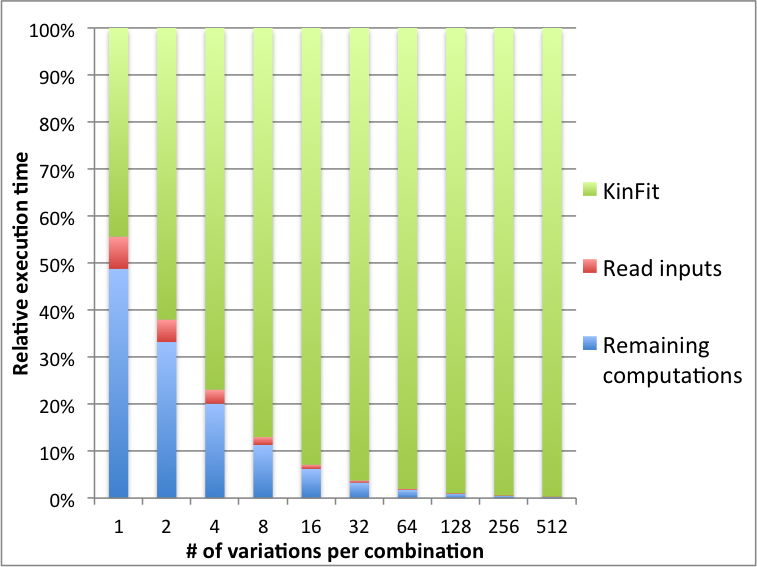
\includegraphics[scale=0.6]{../../common/graphs/relative_exec_time_kinfit_rest.png}  
	%	\captionof{figure}{Another figure}
	%	\label{fig:KinFitGraph2}
	\end{minipage}
	\caption{Absolute (left) and relative (right) execution times for the \tth application considering the \ttDilepKinFit (KinFit) function, I/O and the rest of the computations.}
	\label{fig:KinFitGraph}
\end{figure}

While the I/O and all event processing, with the exception of KinFit, execution times remain constant, with only a slight increase for 256 and 512 variations as it causes more events to be reconstructed, which otherwise would not be possible, and they need to be processed at the final cut 21 (see figure \ref{fig:SchematicFlow1}). As expected, the execution time of KinFit increases linearly with the number of variations to perform per combination. This indicates that the arithmetic intensity of KinFit has the complexity of \textit{O(N)}, where \textit{N} is the number of variations to perform per combination. Consider a given input data file. With no variations, it is possible to consider that the time to process the events remains constant as many times the application is exectued, while using the same input data file. This is the initial problem size. The only way of increasing the problem size, while maintaining the same input data file, is to perform more variations and the number of reconstructions grow linearly with the with this increase. So, for \textit{N} variations it is expected that KinFit execution time will increase by the same factor. This analysis is supported by the experimental data in figure \ref{fig:KinFitGraph}, left graph.

\begin{figure}[!htp]
	\begin{center}
		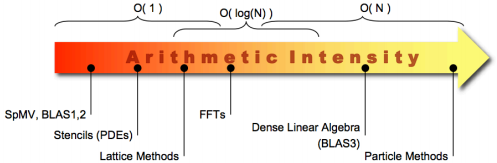
\includegraphics[scale=0.6]{../../common/img/arithmetic_intensity.png}  
		\caption{Arithmetic intensity for various domains of computing problems.}
		\label{fig:ArithmeticIntensity}
	\end{center}
\end{figure}

Figure \ref{fig:ArithmeticIntensity} presents the complexity for various computational purposes. The problems with \textit{O(1)} complexity are not likely to get any benefit from parallelization, opposed to problems with \textit{O(N)} complexity that is more easy to extract performance from parallelization.

The rest of the computational characterization resorted to the analysis of hardware performance counters, using the Performance API \cite{PAPI}, and was performed for the application with no and 256 variations, on the compute-601 system. The instruction mix is presented in figure \ref{fig:InstMix}. By the analysis of the charts is evident that this functions performance cannot be evaluated using the FLOPS metric, as float point operations only account for 14\% and 12\% of the total instructions, for no and 512 variations respectively. \ttDilepKinFit is very diverse in terms of instructions, with loads, branches and stores being the most used. The number of variations does not have a significant impact on the type of instructions issued.

\begin{figure}[!htp]
	\begin{center}
		\raisebox{-0.5\height}{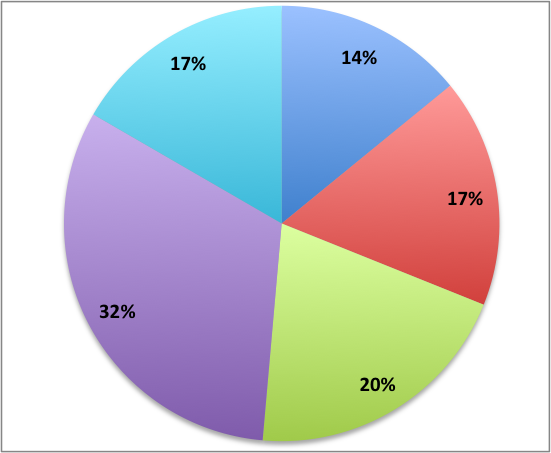
\includegraphics[scale=0.6]{../../common/graphs/inst_mix.png}}
		\raisebox{-0.5\height}{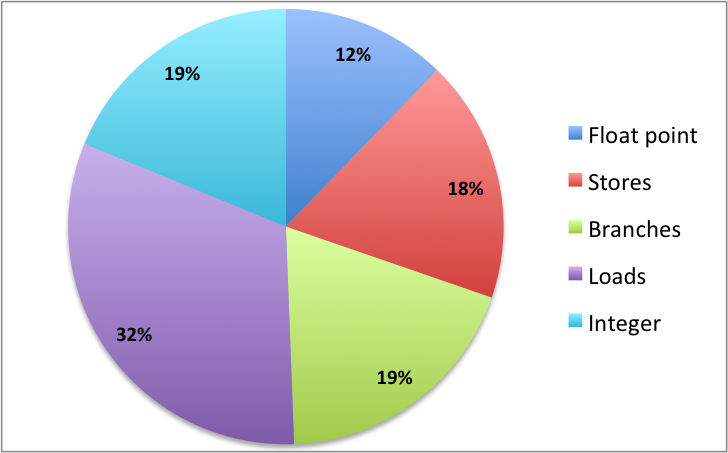
\includegraphics[scale=0.6]{../../common/graphs/inst_mix_256.png}}
		\caption{Instruction mix for the \ttDilepKinFit with no and 512 variations, left and right images respectively.}
		\label{fig:InstMix}
	\end{center}
\end{figure}

The miss rate, for the 3 cache levels, is presented in figure \ref{fig:MissRate}. The miss rate on L1 cache remains constant in 70\% when changing the number of variations. This value is high but it is justified by the huge amount of different computations necessary to reconstruct an event, where data is only reused between one instruction to the other (considering a small scope due to the small cache size), rather than reused by a large set of instructions. The L2 cache miss rate is fairly low and decreases with the number of variations. As it has a larger size than L1 cache, the data is reused more often without causing a miss to the L3 cache. Due to the reuse of data in the L2 cache, and considering the large size of the L3 cache, the miss rate increases with the number of variations. This is not a consequence of a poor cache management but results from the decrease of the L2 cache miss rate, where most L2 cache misses are caused by fetch instructions of new data not yet on cache. The use of more cores, in a shared memory environment, may result in a decrease in the miss rate, specially on L2 cache, as each core will process a smaller set of the data.

\begin{figure}[!htp]
	\begin{center}
		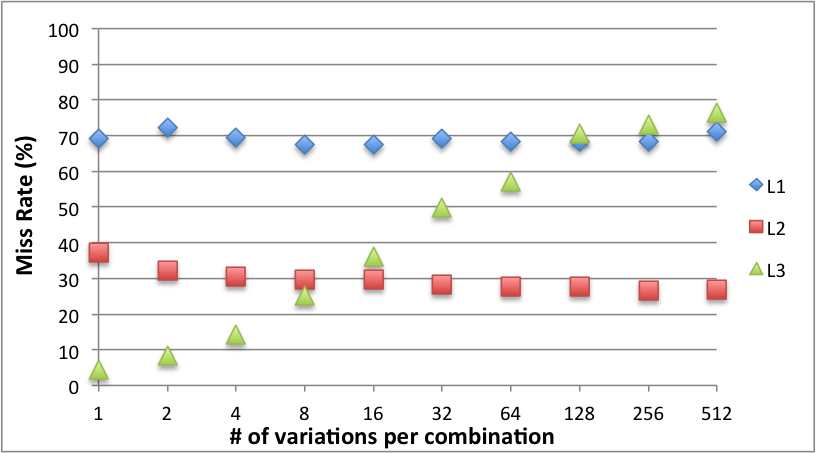
\includegraphics[scale=0.8]{../../common/graphs/miss_rate.png}  
		\caption{Miss rate on L1, L2 and L3 cache of \ttDilepKinFit for various number of variations.}
		\label{fig:MissRate}
	\end{center}
\end{figure}

Operational intensity \cite{Roofline} is a performance metric to characterize the bottlenecks of a given algorithm, based on the assumption that accesses to the system RAM memory are the main performance limitation, also classifying it as memory or compute bound. It requires a Roofline model\footnote{Roofline models for the test systems are presented and explained in appendix \ref{App:Roofline}.} for the system on which the operational intensity is calculated. The operational intensity is the amount of float point operations performed per each byte of data that is fetch from the system RAM memory. However, this is not a reliable metric for this specific problem as only 17\% of the instructions of \ttDilepKinFit is float point arithmetic (refer to chart \ref{fig:InstMix}). Instead, the computational intensity is considered a more reliable metric as it considers all kinds of instructions, with the exception of loads and stores which are not relevant for the algorithm structure.

\begin{figure}[!htp]
	\begin{center}
		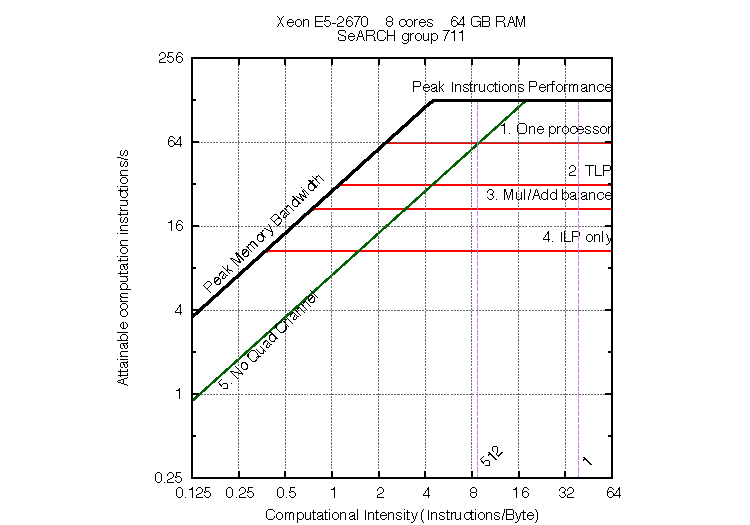
\includegraphics[scale=1]{../../common/601_papi.pdf}  
		\caption{Roofline of the compute-601 system with the computational intensity of \ttDilepKinFit for 1 and 512 variations.}
		\label{fig:Roofline}
	\end{center}
\end{figure}

In figure \ref{fig:Roofline} is presented the Roofline model for the compute-601 system with the computational intensity for \ttDilepKinFit with no and 512 variations. For both number of variations is obvious that this is a compute bound problem, only limited by the peak computational performance of the CPU. This indicates that the optimizations must be focused on increasing the computational throughput rather than on memory accesses. Note that this not include optimizations for accessing the CPU cache.

\subsection{Initial optimizations}
\label{InitialOptimizations}

One limiting factor for the \ttDilepKinFit function is the pseudo-random number generation (PRNG) performed by the \texttt{TRandom} ROOT class, specifically when running a high number of variations, as seen in callgraph \ref{fig:Callgraph256}. From an analysis of the source code is seen that for each variation is needed at most 12 PRNG values. These values are generated and then it is applied a transformation to them so that they follow a Gaussian distribution. The number is generated and transformed by the \texttt{Gauss} function, which occupies 39.4\% of the total execution time. In the input data file used\footnote{See Appendix \ref{App:TestMethodology} for a complete characterization of the test methodology.} there are 1867 events reach the cut 20. This translates in 244056 combinations reconstructed, with a total of 2928672 PRNG values. This is likely to happen with other input data files as each holds a similar number of events. The \texttt{TRandom} generator is being reset with a new seed in every combination, justifying the 23.4\% of execution time for the \texttt{SetSeed} function.

The pseudo-random number generator used by the \texttt{TRandom3} class is the Mersenne Twister \cite{MersenneTwister}, currently one of the most used generators for applications highly dependable on random numbers. This algorithm produces 32-bit uniformly distributed pseudo-random numbers with a period of $2^{19937}$. It has a relatively heavy state which is an integrant part on the algorithm flow. The generator is thread safe as long as different states are being used in different threads. The state can be shared among the threads but, however, changes to it must be done sequentially, serializing the number generation. In this case, the number generated by one thread will affect the number generated by the remaining, and it is not safe to implement in a parallel application.

Since the period of the Mersenne Twister is $2^{19937}$ (approximately $4.3 * 10^{6001}$) and the maximum amount of numbers generated, for 512 variations per combination, is $1.5 * 10^{9}$, it is not necessary to reset the seed of the \texttt{TRandom3} generator, which can reduce the \ttDilepKinFit execution time significantly. Figure \ref{fig:TRandomOptim} illustrates the speedup obtained through this optimization. For a larger number of variations (from 16 to 512) the application is 1.7 to almost 2 times faster, without affecting the credibility of the results.

\begin{figure}[!htp]
	\begin{center}
		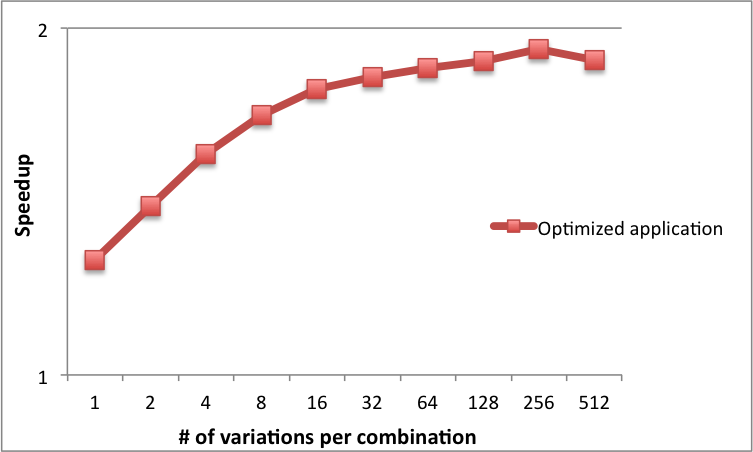
\includegraphics[scale=0.7]{../../common/graphs/speedup_trandom_optim.png}  
		\caption{Speedup of the \tth application with the \texttt{TRandom} optimization.}
		\label{fig:TRandomOptim}
	\end{center}
\end{figure}

\nvidia offers a parallel implementation of the Mersenne Twister for GPUs \cite{NVIDIA:MersenneTwister} in the cuRand library \cite{NVIDIA:cuRand}, important when porting the critical region to run on heterogenous systems with this hardware accelerator. It uses a precomputed set of 200 parameters, which can also be generated by the user, but offering a smaller period of $2^{11213}$. The pseudo-random number generation and state update is thread safe, with up to 256 threads sharing the same state for each block. Two different blocks can safely operate concurrently.

\texttt{TRandom} uses the Acceptance-Complement Ratio algorithm \cite{AcceptanceRandom} for transforming the pseudo-random numbers from an uniform to a gaussian transformation. It is allegely 66\% faster than the Box-Muller transformation \cite{BoxMuller} and similar to the Ziggurat method \cite{Ziggurat}. The cuRand library only offers the Box-Muller transformation with a basic pseudo-random number generator so, to accuratly replicate the results, it is needed to replicate the TRandom gaussian method on GPU using the cuRand implementation of Mersenne Twister.

Other changes were made to the application, dividing the computation of the variations and kinematical reconstruction in modules, in such a way that when developing different parallel versions of \ttDilepKinFit it is easy to switch between them and increase code readbility. Also, the definition of the number of variations to perform is set by environment variables, at runtime, rather than at compile time, easing the user interaction with the application.
